%# -*- coding:utf-8 -*-
\documentclass[10pt,aspectratio=169,mathserif]{beamer}		
%设置为 Beamer 文档类型,设置字体为 10pt,长宽比为16:9,数学字体为 serif 风格

%%%%-----导入宏包-----%%%%
\usepackage{zju}			%导入 zju 模板宏包
\usepackage{ctex}			%导入 ctex 宏包,添加中文支持
\usepackage{amsmath,amsfonts,amssymb,bm}   %导入数学公式所需宏包
\usepackage{color}			 %字体颜色支持
\usepackage{graphicx,hyperref,url}
\usepackage{metalogo}	% 非必须
%% 上文引用的包可按实际情况自行增删
%%%%%%%%%%%%%%%%%%
\usepackage{fontspec}
\usepackage{xeCJK}
\usepackage{multirow}
\usepackage{booktabs}
\usepackage{natbib}
\usepackage{caption}
\captionsetup[figure]{labelformat=empty}
\captionsetup[table]{labelformat=empty}

% \setCJKmainfont{Source Han Sans SC}



\beamertemplateballitem		%设置 Beamer 主题

%%%%------------------------%%%%%
\catcode`\。=\active         %或者=13
\newcommand{。}{.}				
%将正文中的“。”号转换为“.”。中文标点国家规范建议科技文献中的句号用圆点替代
%%%%%%%%%%%%%%%%%%%%%

%%%%----首页信息设置----%%%%
\title[Tokenformer]{TOKENFORMER: RETHINKING TRANSFORMER SCALING WITH TOKENIZED MODEL PARAMETERS}
\subtitle{——Wang et al.,2024}			
%%%%----标题设置


\author[wzl]{
  Li Weizhen \\\medskip}
  %{\small \url{chenqiyuan1012@foxmail.com}} \\
  %{\small \url{https://www.zju.edu.cn/}}}
%%%%----个人信息设置
  
\institute[]{
School of Mathematical Sciences, Zhejiang University }
%%%%----机构信息

\date[Dec. 18 2024]{
  2024.12.18}
%%%%----日期信息
  
\begin{document}

\begin{frame}
	\titlepage
\end{frame}				%生成标题页

%\section{Contents}
\begin{frame}
	\frametitle{Contents}
	\tableofcontents
\end{frame}				%生成提纲页

\section{Introduction}
\begin{frame}
\frametitle{Introduction}
Transformers have become the predominant architecture
in foundation models due to their excellent performance
across various domains. However,
\begin{itemize}
    \item scaling these models requires substantial costs;
    \item architectural modifications typically require the entire
    model to be retrained from scratch.
\end{itemize}
% However, the substantial cost of scaling these models
% remains a significant concern.\\
% When scaling the model, its architectural modifications are introduced
% and the entire model typically requires retraining from scratch.\\
The \textbf{Tokenformer}, a natively scalable architecture that totally
leverages the attention mechanism, was proposed.
\begin{itemize}
    \item Treat model parameters as tokens and replace all linear
    projections in Transformers with token-parameter attention layers;
    \item Input tokens act as queries and model parameters as keys
    and values;
    \item Allow for progressive and efficient scaling without retraining
    from scratch;
    \item Achieve performance comparable to Transformers while
    greatly reducing the training costs.
\end{itemize}
\end{frame}

\begin{frame}
\frametitle{Transformer vs Tokenformer}
\begin{figure}[h]
    \centering
    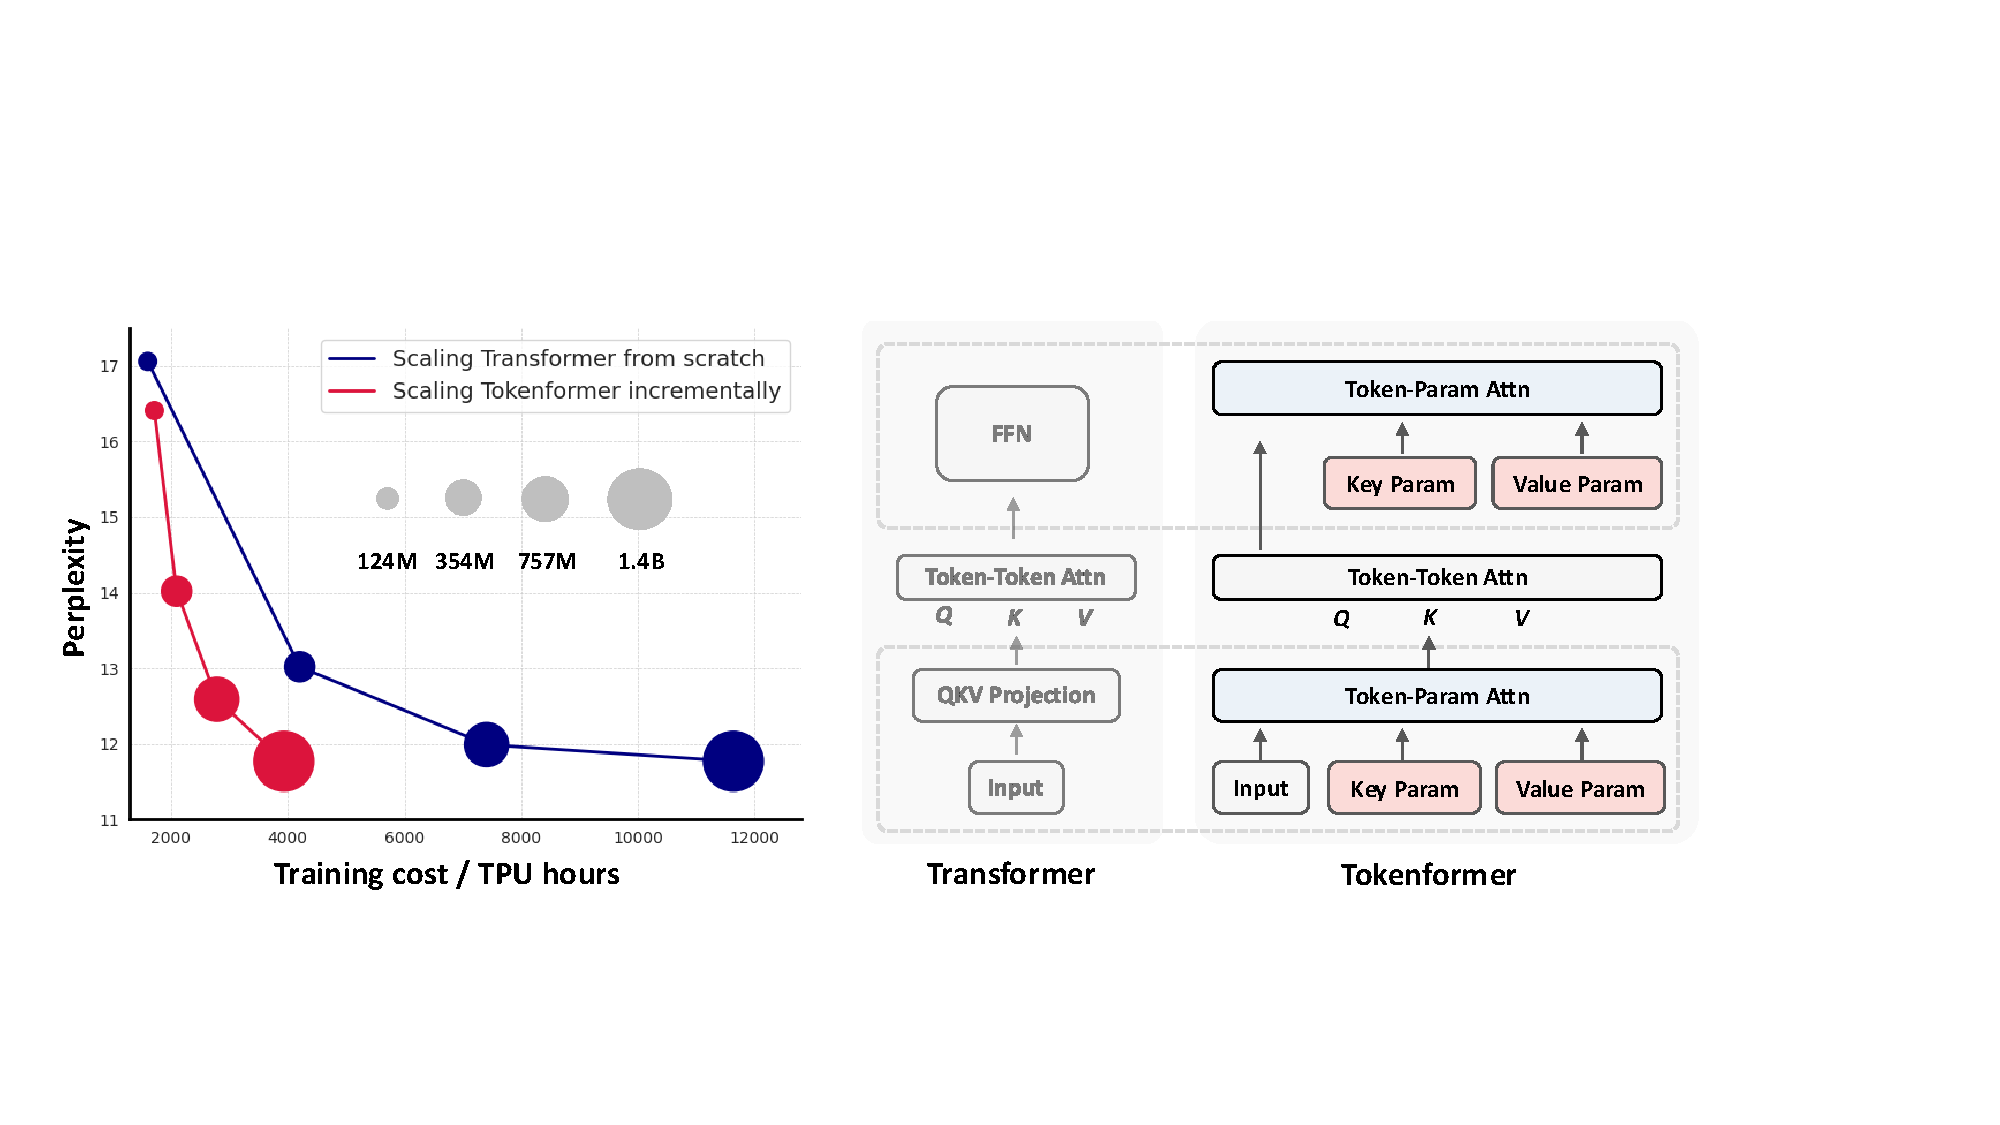
\includegraphics[width=0.99\linewidth]{./transformer-paper/intro_v4.pdf}
    \vspace{-0.1cm}
    \caption{A simple comparasion between Transformers and Tokenformers.}
    \label{fig:intro_figure}
    \vspace{-6pt}
\end{figure}
\end{frame}
\section{Transformer}
\label{sec:transformer}
\begin{frame}
\frametitle{Transformer}
\begin{figure}
    % \begin{minipage}[t]{0.5\textwidth}
    %   \centering
    %   %Scaled Dot-Product Attention \\
    %   Transformer model architecture \\
    %   \vspace{0.1cm}
    %   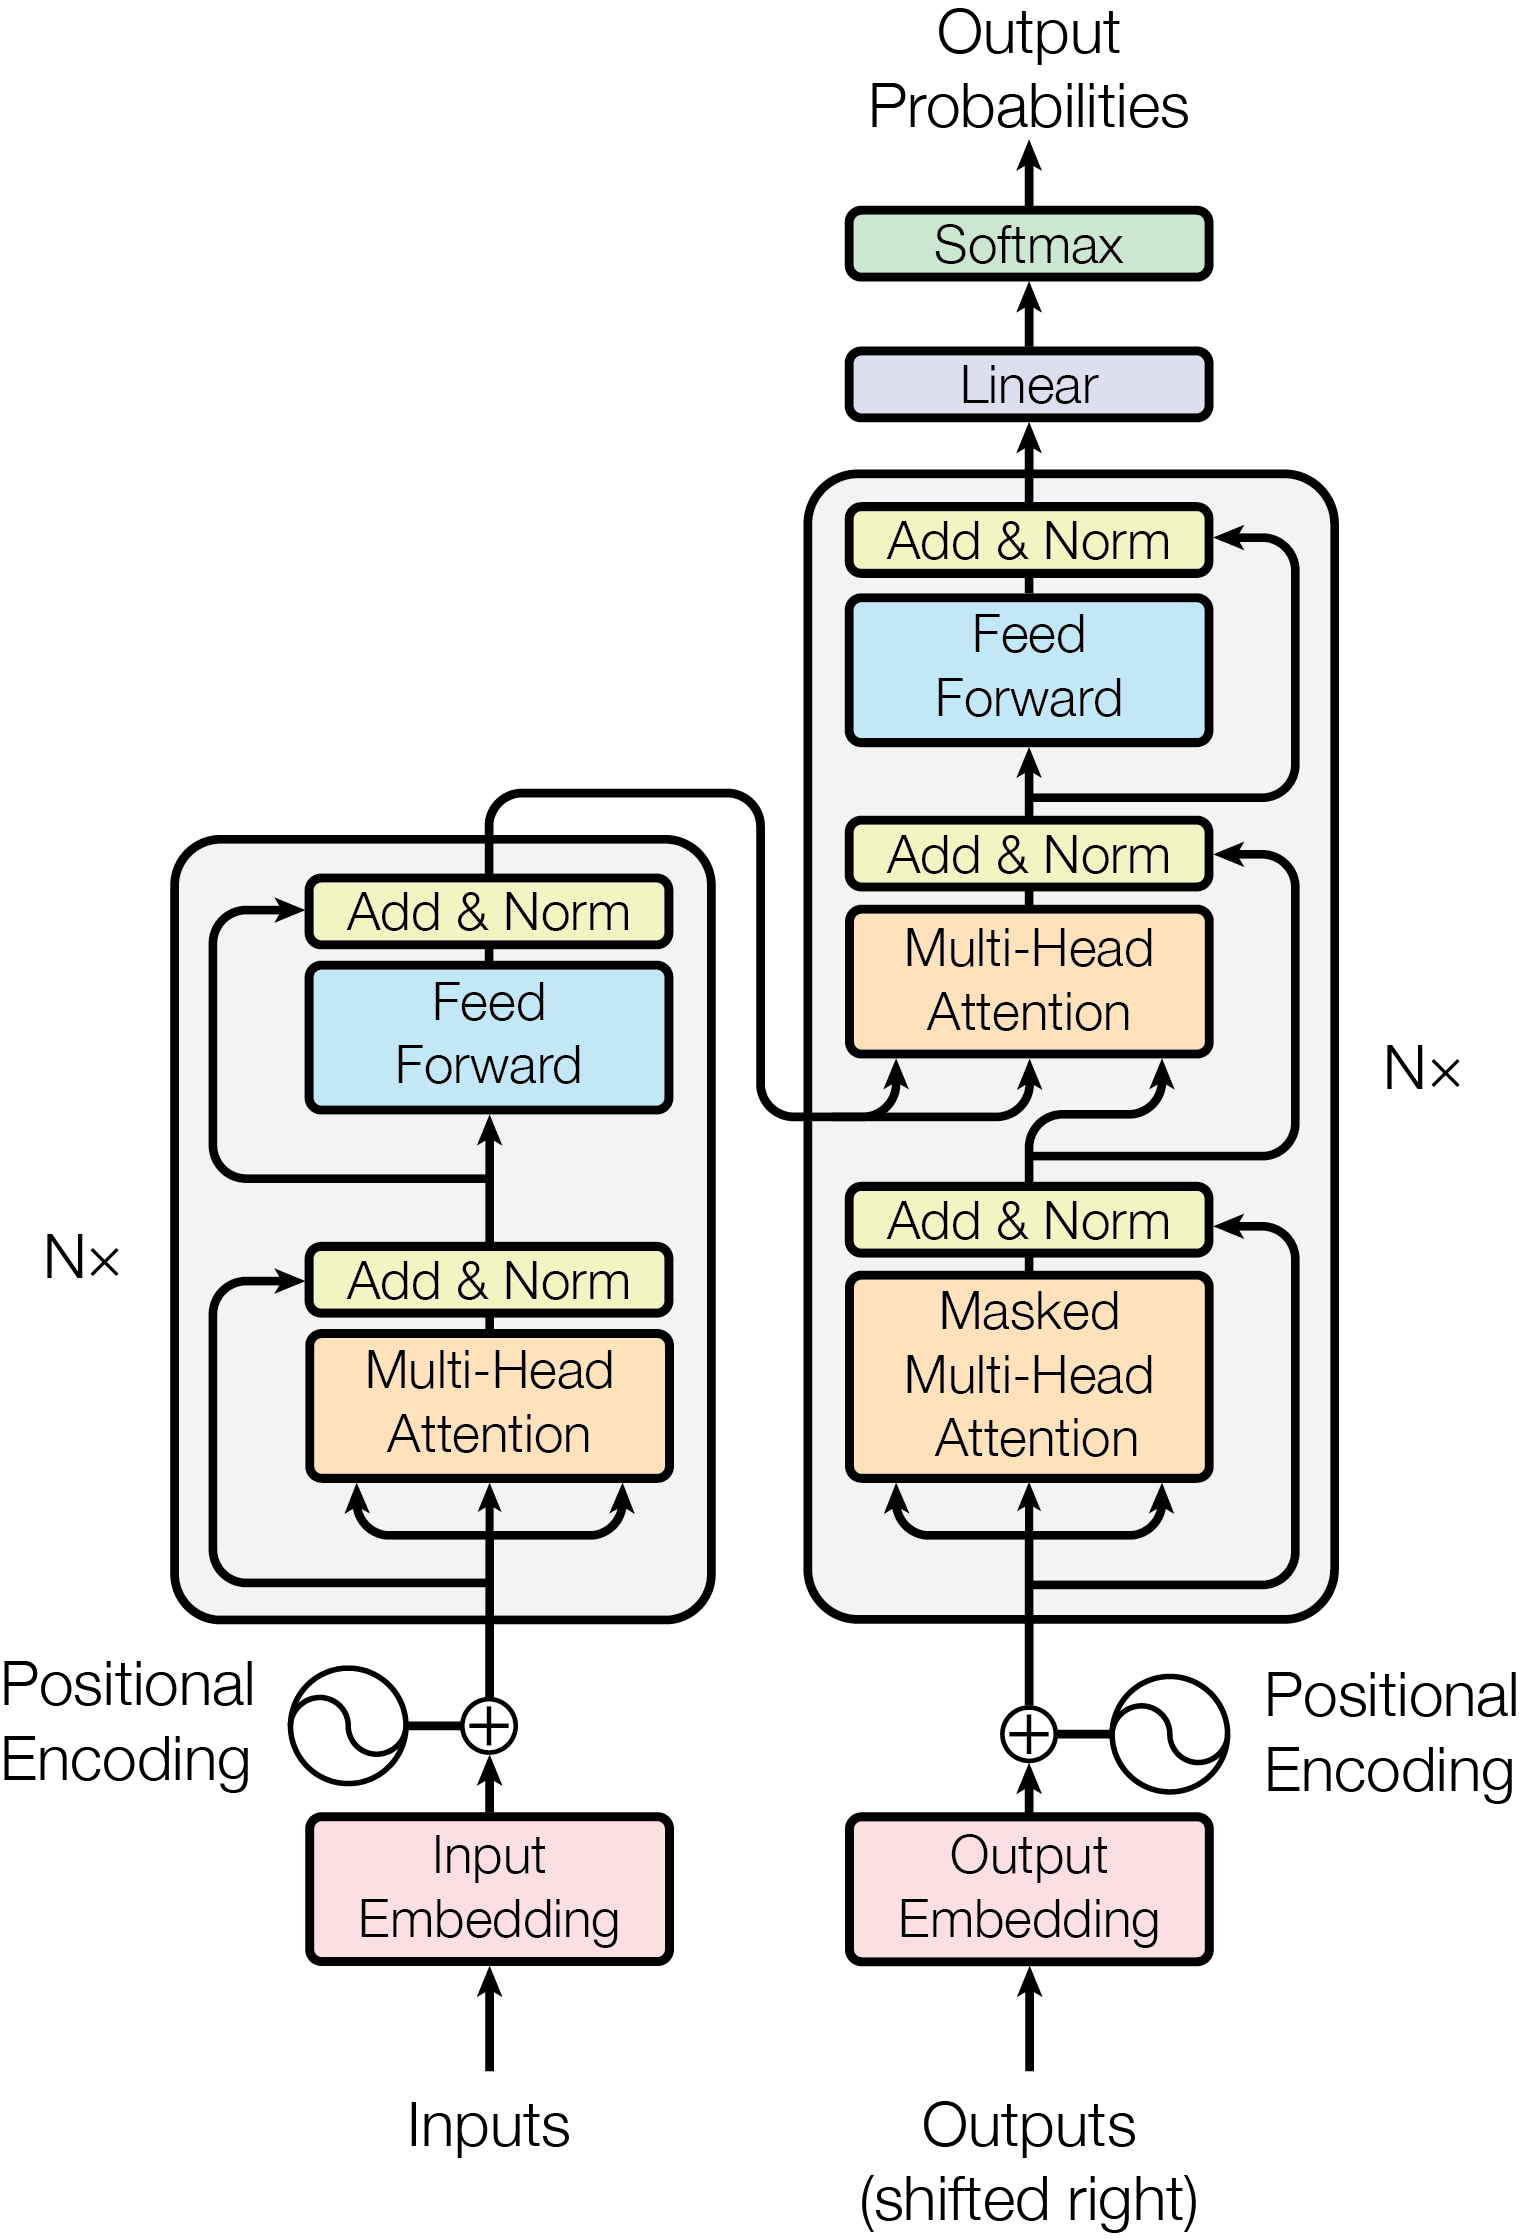
\includegraphics[scale=0.35]{./tokenformer-paper/Figures/ModalNet-21}
    % \end{minipage}\hfill
    \begin{minipage}[t]{0.5\textwidth}
      \centering 
      Multi-Head Attention \\
      \vspace{0.1cm}
      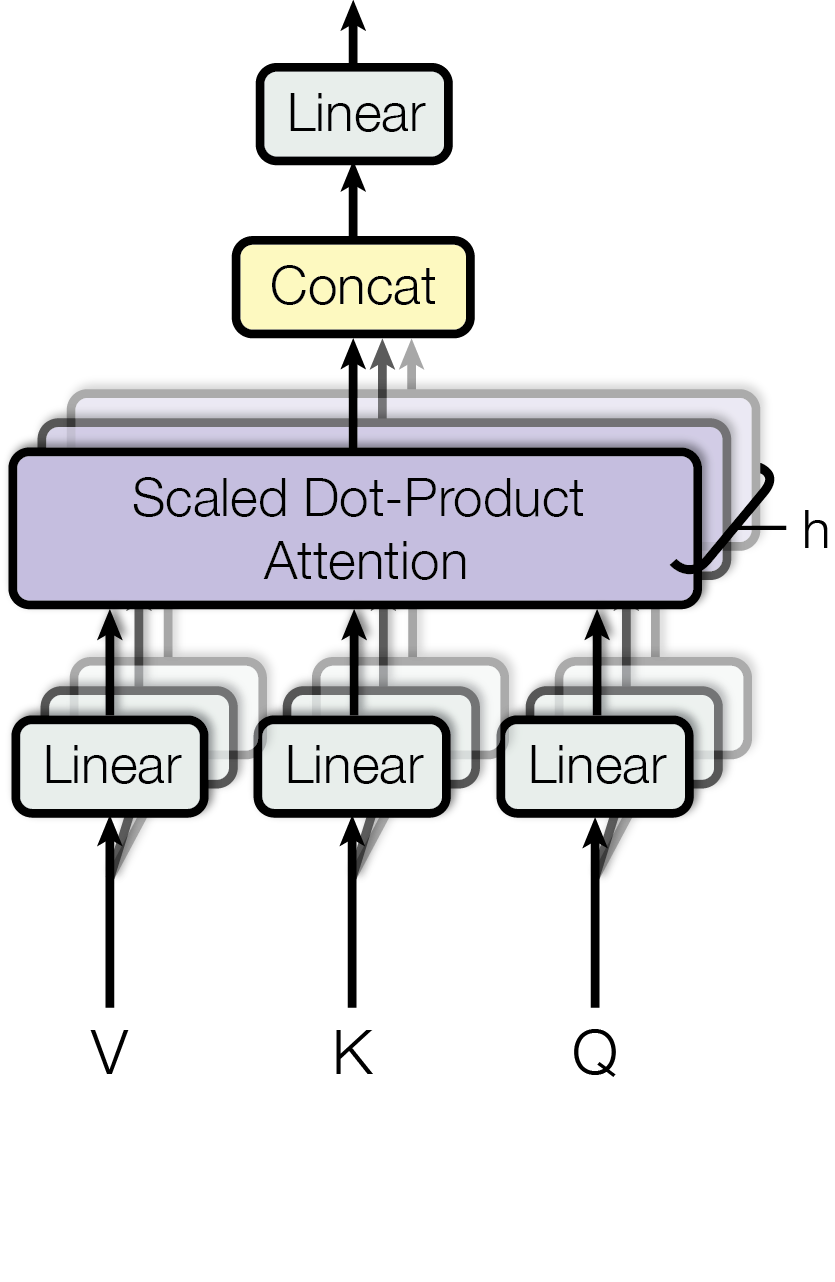
\includegraphics[scale=0.6]{./tokenformer-paper/Figures/ModalNet-20}  
    \end{minipage}\hfill
    \begin{minipage}[t]{0.5\textwidth}
      %\centering 
       Input tokens: $X\in\mathbb{R}^{T\times d}$ \\
       \begin{equation}
        Q = X\cdot W^Q, \quad K = X\cdot W^K, \quad V = X\cdot W^V;
       \end{equation}
       $W^Q, W^K \in\mathbb{R}^{d\times d_k}, W^V \in\mathbb{R}^{d\times d_v}$. \\
       \begin{equation}
        \text{Attention}(Q,K,V)=\text{softmax}(\frac{QK^T}{\sqrt{d_k}})V.
       \end{equation}
       Output: $$O=X_{\text{att}}\cdot W^O, \quad W^O \in\mathbb{R}^{d_v\times d}.$$
       FFN: $$X_{\text{ffn}} = \text{Activation}(O\cdot W_1 + b_1)W_2 + b_2.$$
       $W_1 \in \mathbb{R}^{d\times d_{\text{ffn}}},
       W_2 \in \mathbb{R}^{d_{\text{ffn}}\times d}.$
    \end{minipage}
    
    
      % \centering
    
      %\caption{(left) Scaled Dot-Product Attention. (right) Multi-Head Attention consists of several attention layers running in parallel.}
      \label{fig:multi-head-att}
    \end{figure}
    
\end{frame}

\section{TokenFormer}
\label{sec:tokenformer}
\begin{frame}
\frametitle{TokenFormer}
\begin{figure}[h]
    \centering
    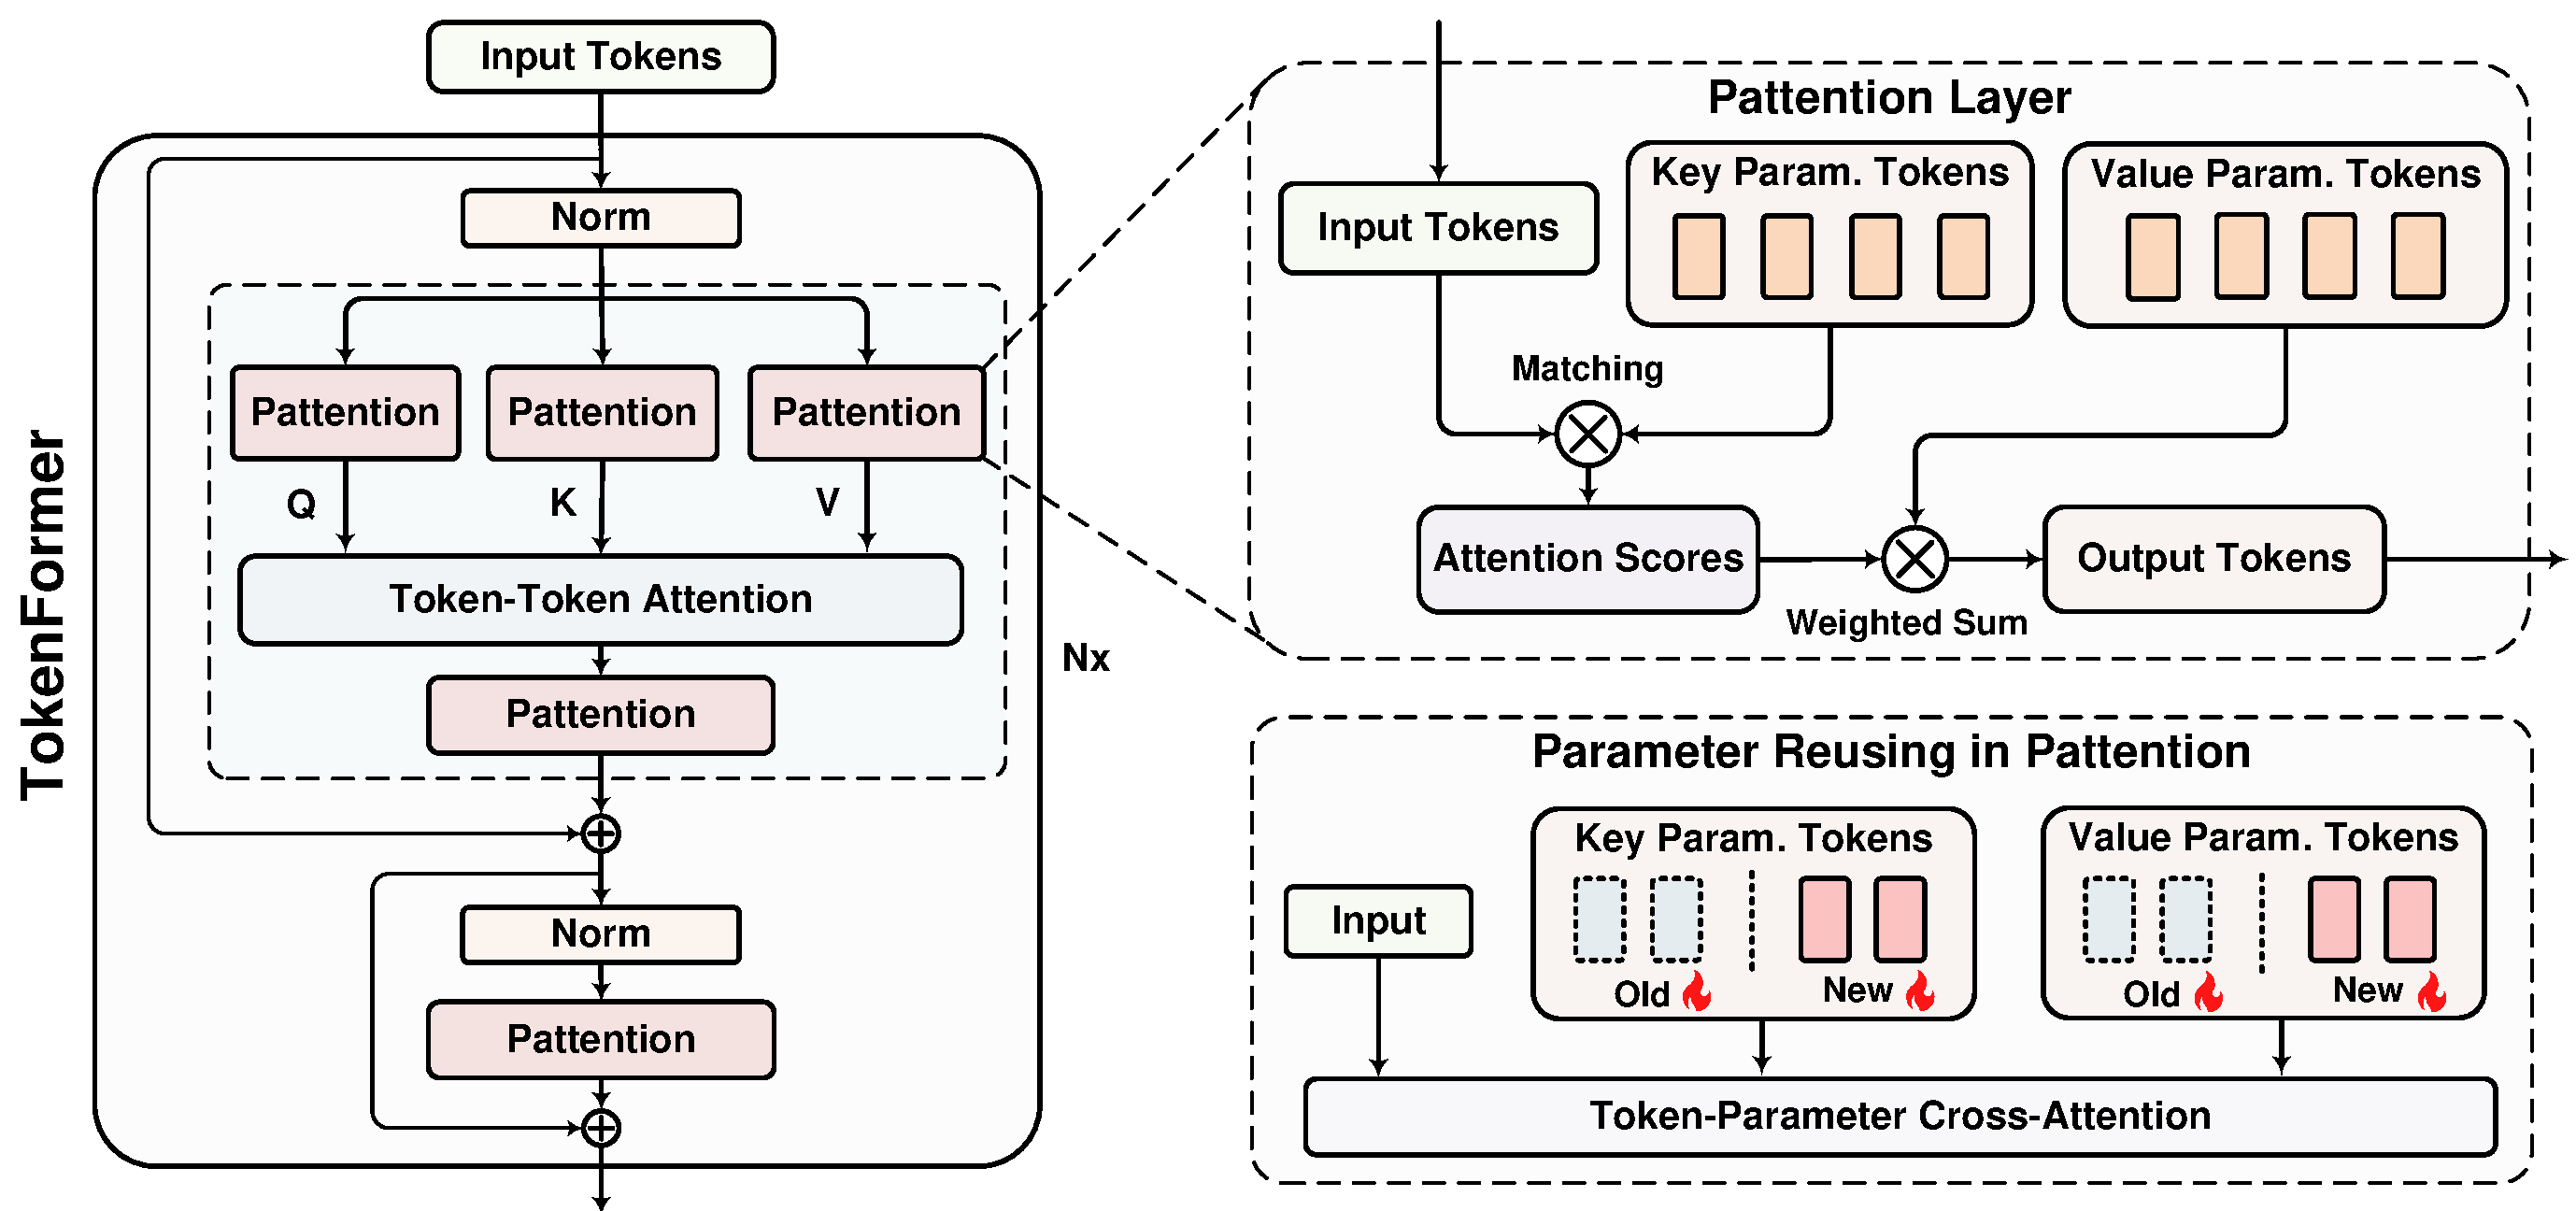
\includegraphics[width=0.99\linewidth]{./transformer-paper/arch2.pdf}
    \vspace{-0.1cm}
    \label{fig:tokenformer_figure}
    \vspace{-6pt}
\end{figure}
\end{frame}

\begin{frame}
\frametitle{Pattention Layer}
Let $K_P\in \mathbb{R}^{n\times d_1}$ and $V_P\in \mathbb{R}^{n\times d_2}$
represent the learnable parameter tokens.($n$ is the number of key-value pairs)
\begin{equation}
    \text{Pattention}(X,K_P,V_P)=\theta(X\cdot K_P^T)\cdot V_P,
\end{equation}
where $\theta$ is the modified softmax function. The output Pattention
scores, $S\in \mathbb{R}^{n\times n}$, are computed as:
\begin{equation}
    S_{ij} = \text{GeLU}\left(\frac{A_{ij} \times \tau}{\sqrt{\sum_{k=1}^n |A_{ik}|^2}}\right),
    ~~\forall~i,j \in 1...n,
\end{equation}
where $A=X\cdot K_P^T$ and $\tau$ is a scale factor.\\ \vspace{5pt}
In transformer, we have $Q=X\cdot W_Q$.\\
In tokenformer, we have $Q=\text{Pattention}(X,K_P^Q,V_P^Q)$.
\end{frame}

\begin{frame}
\frametitle{Overall Architecture}
\begin{itemize}
    \item QKV Pattention:$$Q=\text{Pattention}(X,K_P^Q,V_P^Q),~~
    K = \text{Pattention}(X,K_P^K,V_P^K),~~ V = \text{Pattention}(X,K_P^V,V_P^V).$$
    \item Token-Token Attention:
    $$X_{\text{att}}=\text{softmax}\left(\frac{Q\cdot K^T}{\sqrt{d}}\right)\cdot V,$$
    $$O_{\text{att}}=\text{Pattention}(X_{\text{att}},K_P^O,V_P^O).$$
    \item FFN:
    $$O_{\text{ffn}}=\text{Pattention}(O_{\text{att}},K_P^{\text{ffn}},V_P^{\text{ffn}}).$$
\end{itemize}
\end{frame}

\begin{frame}
\frametitle{Progressive Model Scaling}
Consider an existing Tokenformer model equipped with a
set of pre-trained key-value parameter tokens,
denoted as $K_P^{\text{old}}, V_P^{\text{old}} \in \mathbb{R}^{n \times d}$.
To scale the model, just augment this set by appending new key-value parameter
tokens $K_P^{\text{new}}, V_P^{\text{new}} \in \mathbb{R}^{m \times d}$ as
\begin{equation}
    K_P^{\text{scale}} = \left[K_P^{\text{old}}, K_P^{\text{new}}\right],
    ~~~~~V_P^{\text{scale}} = \left[V_P^{\text{old}}, V_P^{\text{new}}\right].
\end{equation}
\begin{equation}
    O = \text{Pattention}\left(X, K_P^{\text{scale}}, V_P^{\text{scale}}\right).
    \label{eq:token-parameter-3}
\end{equation}
Importantly, by initializing $K^{\text{new}}_P$ with zero,
the model can perfectly resume the model state from the pre-training
phase without losing the well-learned knowledge,
facilitating faster convergence and accelerating the overall scaling process.

\end{frame}
\section{Experiments}
\begin{frame}
\frametitle{Experiments---Progressive Modeling Scaling}
\begin{figure}[h]
    \centering
    \begin{minipage}{0.49\linewidth}
        \centering
        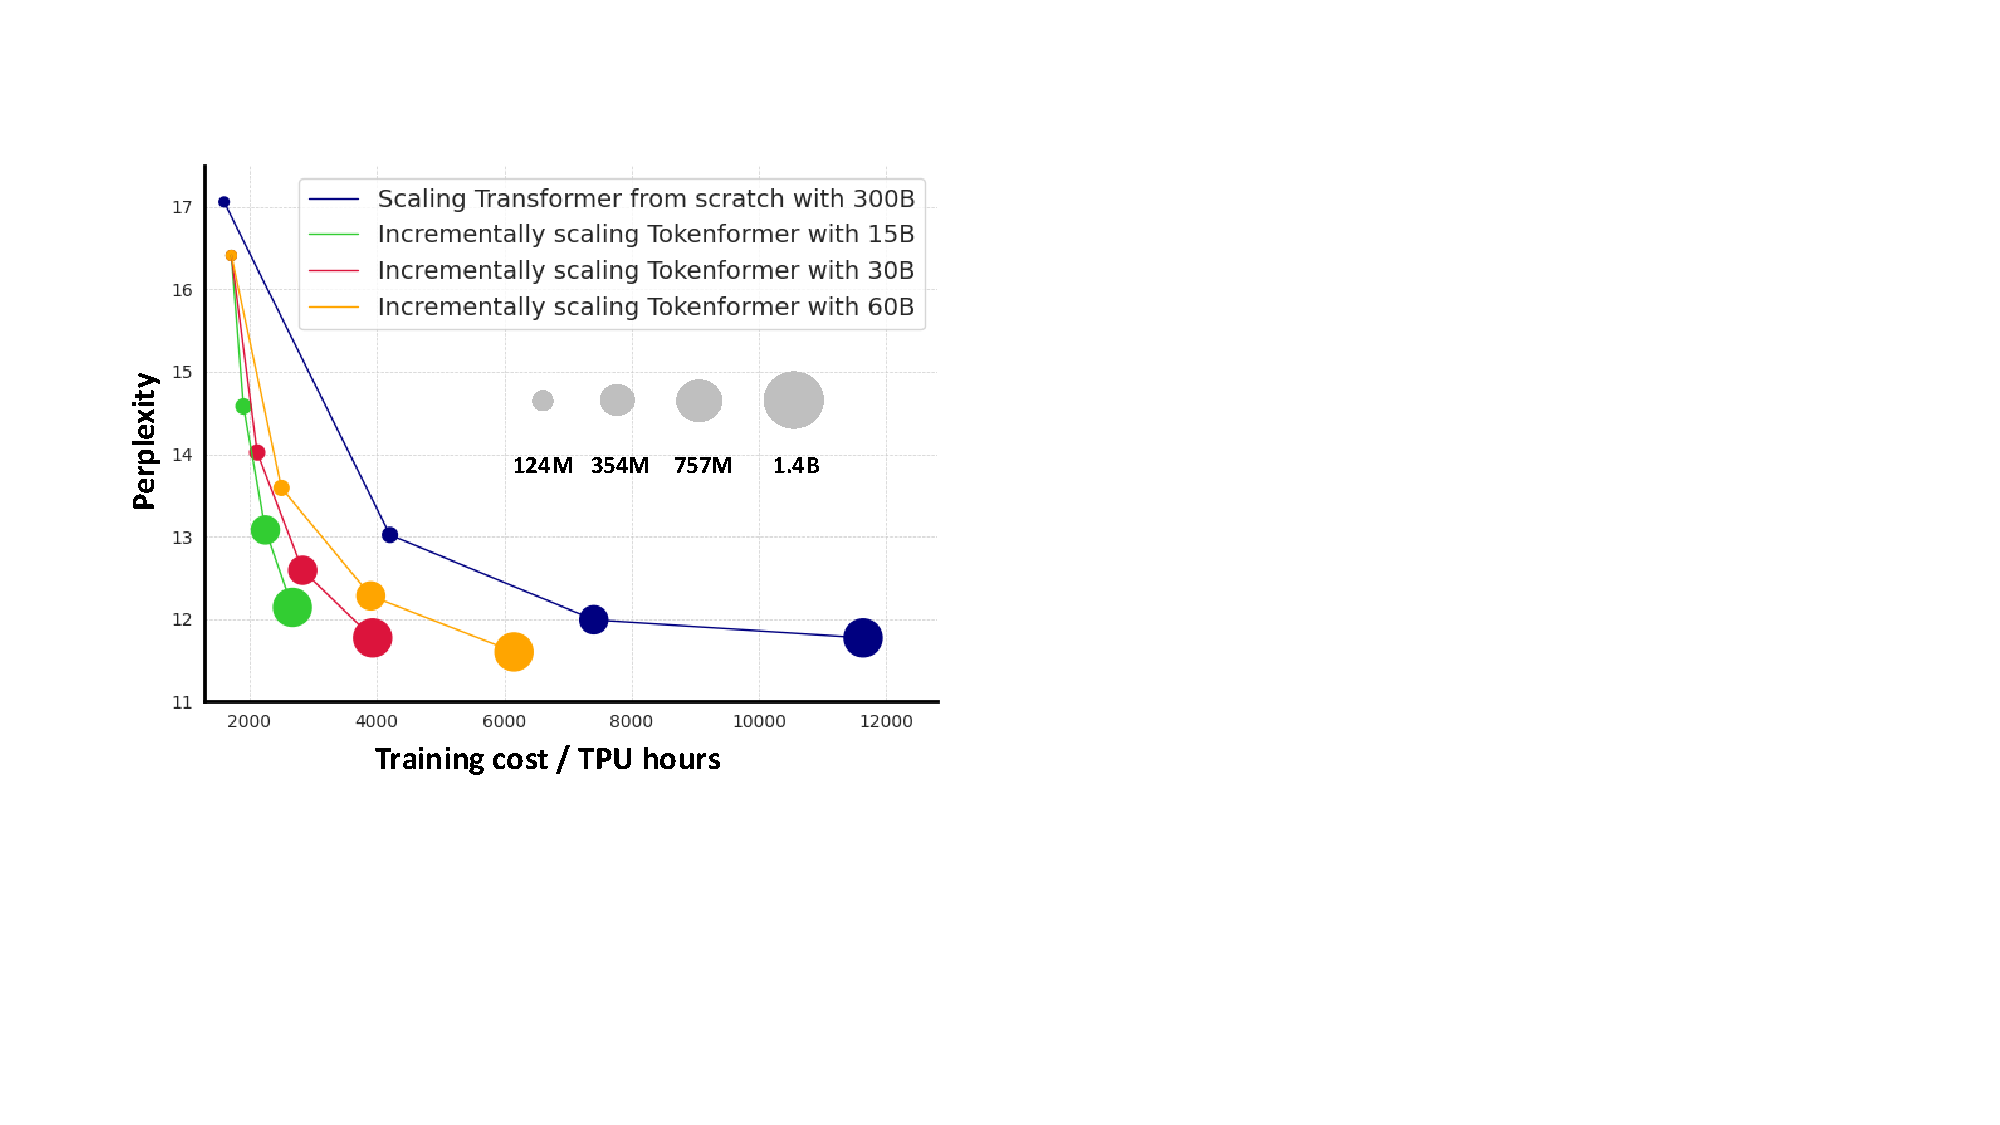
\includegraphics[width=1.0\linewidth]{./transformer-paper/main_results_v2_left.pdf}
        %\vspace{-16pt}
        %\caption{Evaluating model scaling costs through cumulative computational budgets. The Transformer baseline incurs expenses for each individual scaling step performed independently from scratch, whereas \ourmethod aggregates costs across all scaling stages, including training a 124M model initially, progressively scaling to 354M, 757M, and 1.4B parameters.}
        \label{fig:scaling_accum}
    \end{minipage}
    \hfill
    \begin{minipage}{0.49\linewidth}
        \centering
        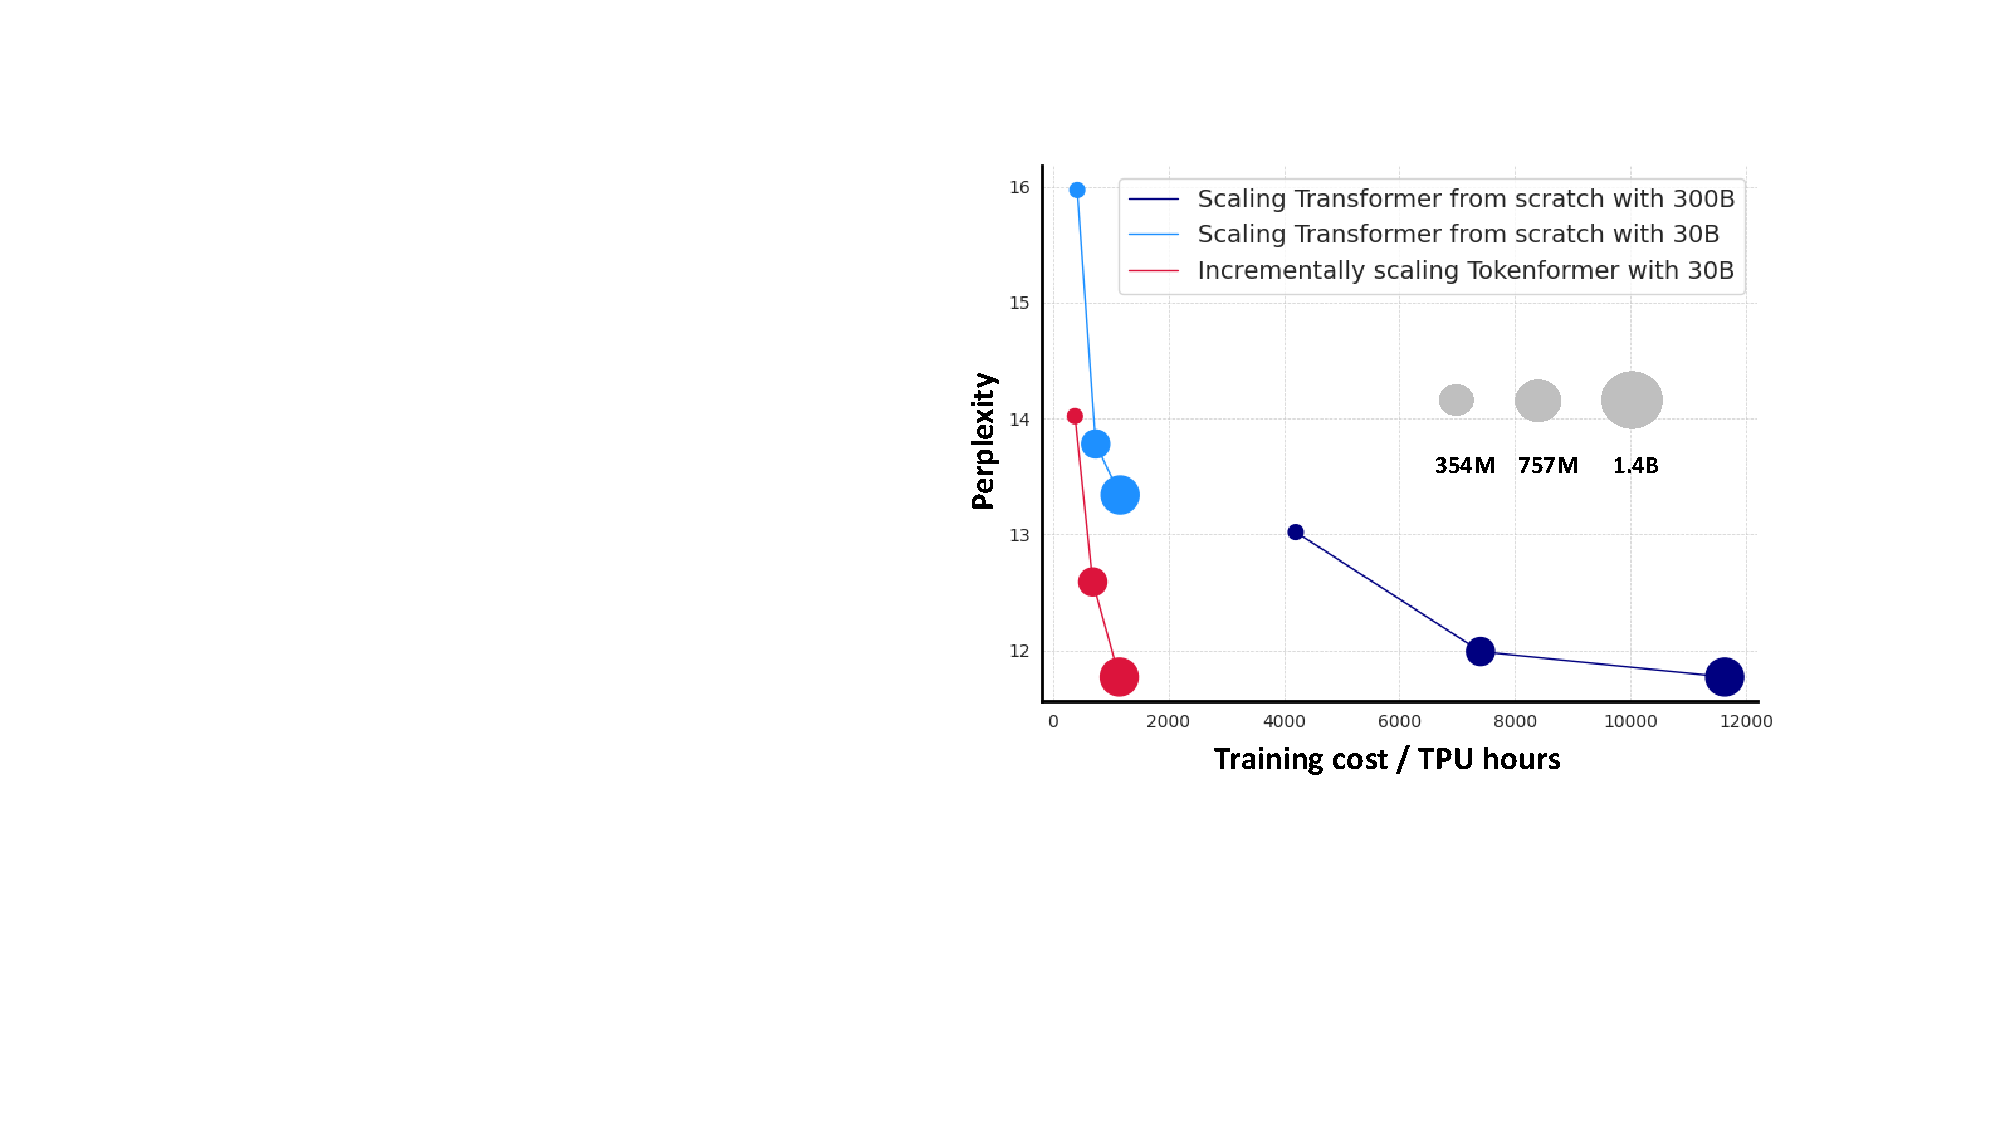
\includegraphics[width=1.0\linewidth]{./transformer-paper/main_results_v2_right.pdf}
        %\vspace{-16pt}
        %\caption{Evaluating model scaling costs by measuring the budget required at each scaling stage. The Transformer baselines used are consistent with those depicted in Figure~\ref{fig:scaling_accum}, trained with 30B and 300B tokens. Similarly, for \ourmethod, the cost is the budget required for each incremental scaling step from a smaller one. All the experiments were conducted on TPU v4 hardware.}
        \label{fig:scaling_individual}
    \end{minipage}
\end{figure}
\end{frame}

\begin{frame}
\frametitle{Experiments---Benchmarking}
\begin{table}[t]
    \centering
    \resizebox{\textwidth}{!}{
    \begin{tabular}{cccccccccc|c}
      \toprule
      & & Pile & LAMBADA & LAMBADA & HellaSwag & PIQA & Arc-E & Arc-C & WinoGrande & Average \\
      \multirow{-2}{*}{Model}     & \multirow{-2}{*}{\#Param}    & ppl $\downarrow$ & ppl $\downarrow$ & acc $\uparrow$ & acc $\uparrow$ & acc $\uparrow$ & acc $\uparrow$ & acc $\uparrow$  & acc $\uparrow$ & acc $\uparrow$\\
      \midrule
      Pythia-160M 			& 160M	   & 29.64 & 37.25 & 35.4 & 30.3 & 62.3 & 43.6 & 23.6 & \textbf{51.3} & 40.1\\
      \textbf{Ours (TokenFormer-150M)} & 150M & \textbf{10.45} & \textbf{16.38} & \textbf{45.0} & \textbf{35.5} & \textbf{64.9} & \textbf{47.3} & \textbf{24.9} & 50.4 & \textbf{44.7}\\
      \midrule
      Pythia-410M 			& 410M	   & 9.95 & 10.84 & 51.4 & 40.6 & 66.9 & 52.1 & 24.6 & 53.8 & 48.2\\
      \textbf{Ours (TokenFormer-450M)}			    & 450M	   & \textbf{8.28} & \textbf{7.69} & \textbf{57.3} & \textbf{47.5} & \textbf{69.5} & \textbf{56.2} & \textbf{26.7} & \textbf{54.6} & \textbf{52.0}\\
      \midrule
      Pythia-1B 			& 1B	   & 7.82 & 7.92 & 56.1 & 47.2 & 70.7 & 57.0 &  27.1 &  53.5 & 51.9\\
      \textbf{Ours (TokenFormer-900M)}			    & 900M	   & \textbf{7.38} & \textbf{5.46} & \textbf{64.0} & \textbf{55.3} & \textbf{72.4} & \textbf{59.9} &  \textbf{30.6} &  \textbf{56.4} & \textbf{56.4} \\
      \midrule
      GPT-Neo 1.3B           & 1.3B     &  -   &7.50 & 57.2 & 48.9 & 71.1 & 56.2 & 25.9 & 54.9 & 52.4 \\
      OPT-1.3B            & 1.3B     &  -   &6.64 & 58.0 & 53.7 & 72.4 & 56.7 & 29.6 & 59.5 & 55.0 \\
      Pythia-1.3B			& 1.3B	   & 7.51 &6.08 & 61.7 & 52.1 & 71.0 & 60.5 &  28.5 &  57.2 & 55.2\\
      GPT-Neo 2.7B            & 2.7B     &  -   &5.63 & 62.2 & 55.8 & 71.1 & 61.1 & 30.2  & 57.6 & 56.5\\
      OPT-2.7B            & 2.7B     &  -   &5.12 & 63.6 & \textbf{60.6} & 74.8 & 60.8 & 31.3 & \textbf{61.0} & 58.7\\
      Pythia-2.8B			& 2.8B	   & - &\textbf{5.04} & 64.7 & 59.3 & 74.0 & 64.1 &  \textbf{32.9} &  59.7 & 59.1\\
      \hline
      \textbf{Ours (TokenFormer-1.5B)}			& 1.5B	   & \textbf{6.91} & 5.24 & \textbf{64.7} & 60.0 & \textbf{74.8} & \textbf{64.8} &  32.0 & 59.7 & \textbf{59.3} \\
      \bottomrule
    \end{tabular}
    } 
    %\vspace{-8pt}
      \caption{\textbf{Zero-shot Evaluations.}}
      % The best performance for each model size is highlighted in bold. Our comparisons are made with publicly available transformer-based LMs with various tokenizers. Following Pythia~\citep{biderman2023pythia}, our model is trained for up to 300B tokens on pile dataset. }
      \label{tab:llm_benchmark}
  \end{table}
\end{frame}

\begin{frame}
\frametitle{Experiments---Benchmarking}
\begin{table}[t]
    \vspace{-2pt}
    \centering
    \resizebox{0.6\textwidth}{!}{
    \begin{tabular}{cccccccccc}
      \toprule
     Method & Image Size &  \#Param&Top-1 acc \\
      \midrule
      ViT-B/16 			& 384$^2$ & 86M  & 77.9\\
      DeiT-B/16			& 224$^2$ & 86M  & 81.8\\
      ViT-B/16~(MAE) 			& 224$^2$ & 86M  & 82.3\\
      Ours (TokenFormer-B/16$^{\dag}$ )			& 224$^2$ & 86M  & 82.1\\
      \textbf{Ours (TokenFormer-B/16)}			& 224$^2$ & 109M & \textbf{82.5}\\
      \midrule
      ViT-L/16 			& 384$^2$ & 307M & 76.5\\
      ViT-L/16~(MAE)			& 224$^2$ & 307M & 82.6\\
      Ours (TokenFormer-L/16$^{\dag}$)			& 224$^2$ & 307M & 83.0 \\
      \textbf{Ours (TokenFormer-L/16)}			& 224$^2$ & 407M & \textbf{83.1} \\
      \bottomrule
    \end{tabular}
    }
  \caption{\textbf{Image Classification.}} 
  %Comparison of standard vision transformer on ImageNet-1K. The training hyperparameters are completely consistent~(batch size, learning rate, etc.) with \citet{he2022masked}. $\dag$ denotes models where the parameter size has been matched to that of the standard ViT.}
  \label{tab:visual_benchmark}
  %\vspace{-8pt}
\end{table}
\end{frame}

\begin{frame}
\frametitle{Experiments---Comparison with Transformer}
\begin{table}[h]
  \centering
  \resizebox{\textwidth}{!}{
  \begin{tabular}{lcc|cc}
    \toprule
    & \multicolumn{2}{c}{Parameter~~~~~~~~~~~~~~~} & \multicolumn{2}{c}{Training FLOPs}\\
    \multirow{-2}{*}{Operation} & Transformer & Ours & Transformer & Ours \\
    \midrule
    Embed  		& $n_{\text{vocab}}d_{\text{model}}$  & $n_{\text{vocab}}d_{\text{model}}$ & - & -\\
    Attention: QKV Project  		& $3n_{\text{layer}}d_{\text{model}}^2$  & $n_{\text{layer}}d_{\text{token}}(n_{\text{q}}+ n_{\text{k}} + n_{\text{v}}$)& $6n_{\text{layer}}d_{\text{model}}^2T$& $2n_{\text{layer}}d_{\text{token}}(n_{\text{q}}+ n_{\text{k}} + n_{\text{v}})T$\\
    Attention: Token-Token 		& - & - & $4n_{\text{layer}}d_{\text{model}}T^2$ & $4n_{\text{layer}}d_{\text{token}}T^2$ \\
    Attention: Output Project      & $n_{\text{layer}}d_{\text{model}}^2$ & $n_{\text{layer}}d_{\text{token}}n_{\text{o}}$ & $2n_{\text{layer}}d_{\text{model}}^2T$ & $2n_{\text{layer}}d_{\text{token}}n_{\text{o}}T$\\
    Feedforward          & $8n_{\text{layer}}d_{\text{model}}^2$   & $2n_{\text{layer}}d_{\text{token}}n_{\text{ff}}$ & $16n_{\text{layer}}d_{\text{model}}^2T$ & $4n_{\text{layer}}d_{\text{token}}n_{\text{ff}}T$\\
    De-embed  		& - & - & 2$n_{\text{vocab}}d_{\text{model}}$ & 2$n_{\text{vocab}}d_{\text{model}}$\\
    \midrule
    Total~(Non-Embedding)           & $N=12n_{\text{layer}}d_{\text{model}}^2$    & $N=n_{\text{layer}}d_{\text{token}}(n_{\text{q}}+n_{\text{k}}+n_{\text{v}}+n_{\text{o}}+2n_{\text{ff}})$ & $2NT + 4n_{\text{layer}}d_{\text{model}}T^2$ & $2NT + 4n_{\text{layer}}d_{\text{token}}T^2$ \\
    \bottomrule
  \end{tabular}
  }
    \caption{Parameter counts and training compute estimates for Transformer and Tokenformer.}
    \label{tab:flops_and_param}
\end{table}
\end{frame}

\begin{frame}
\frametitle{Experiments---Comparison with Transformer}
\begin{figure}[h]
  \centering
  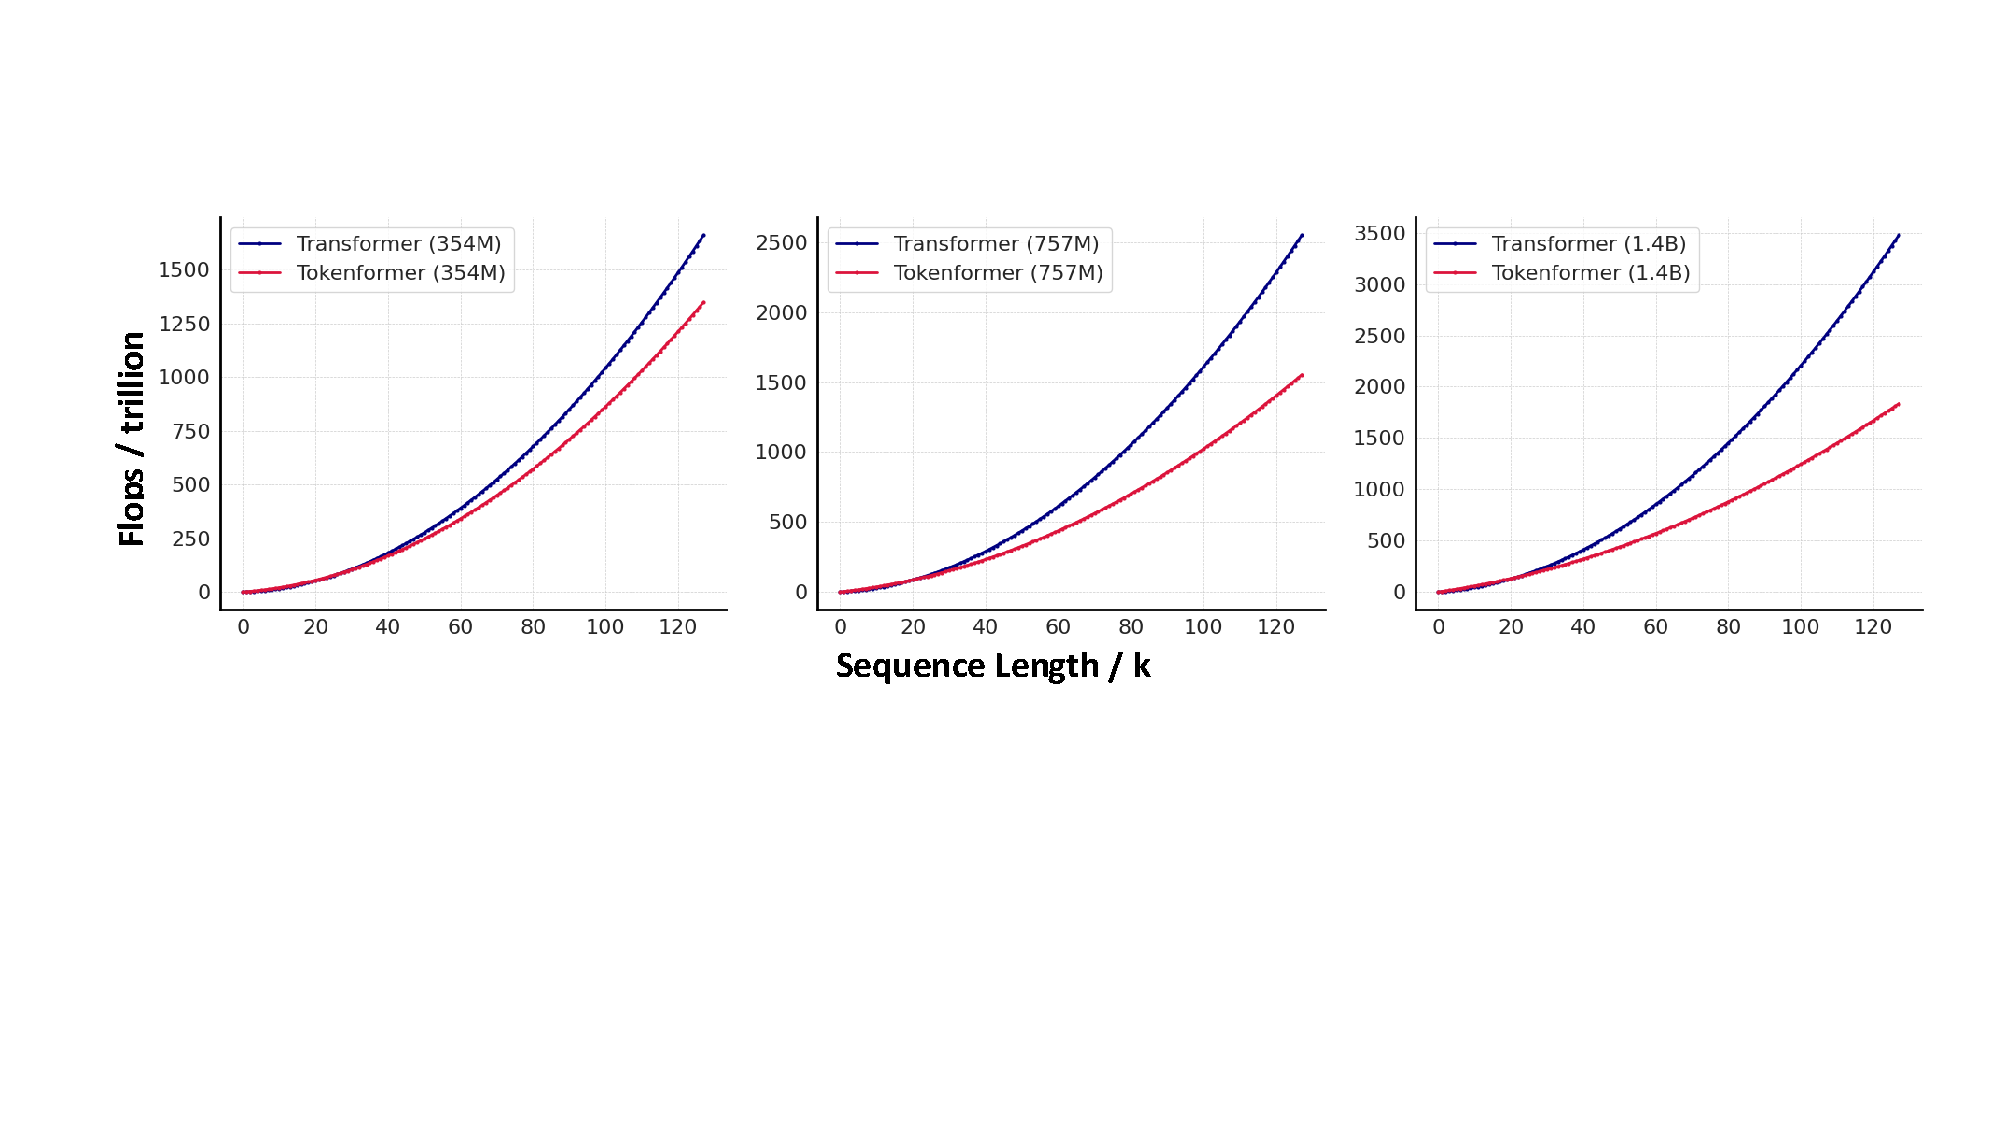
\includegraphics[width=\linewidth]{./transformer-paper/flops_figure.pdf}
  \caption{The relationship between FLOPs and text length for both Transformer and Tokenformer.}
    \label{fig:flops_figure}
\end{figure}
\end{frame}

\begin{frame}
\frametitle{Experiments---Comparison with Transformer}
\begin{figure}[t]
  \centering
  \begin{minipage}{0.49\textwidth}
      \centering
      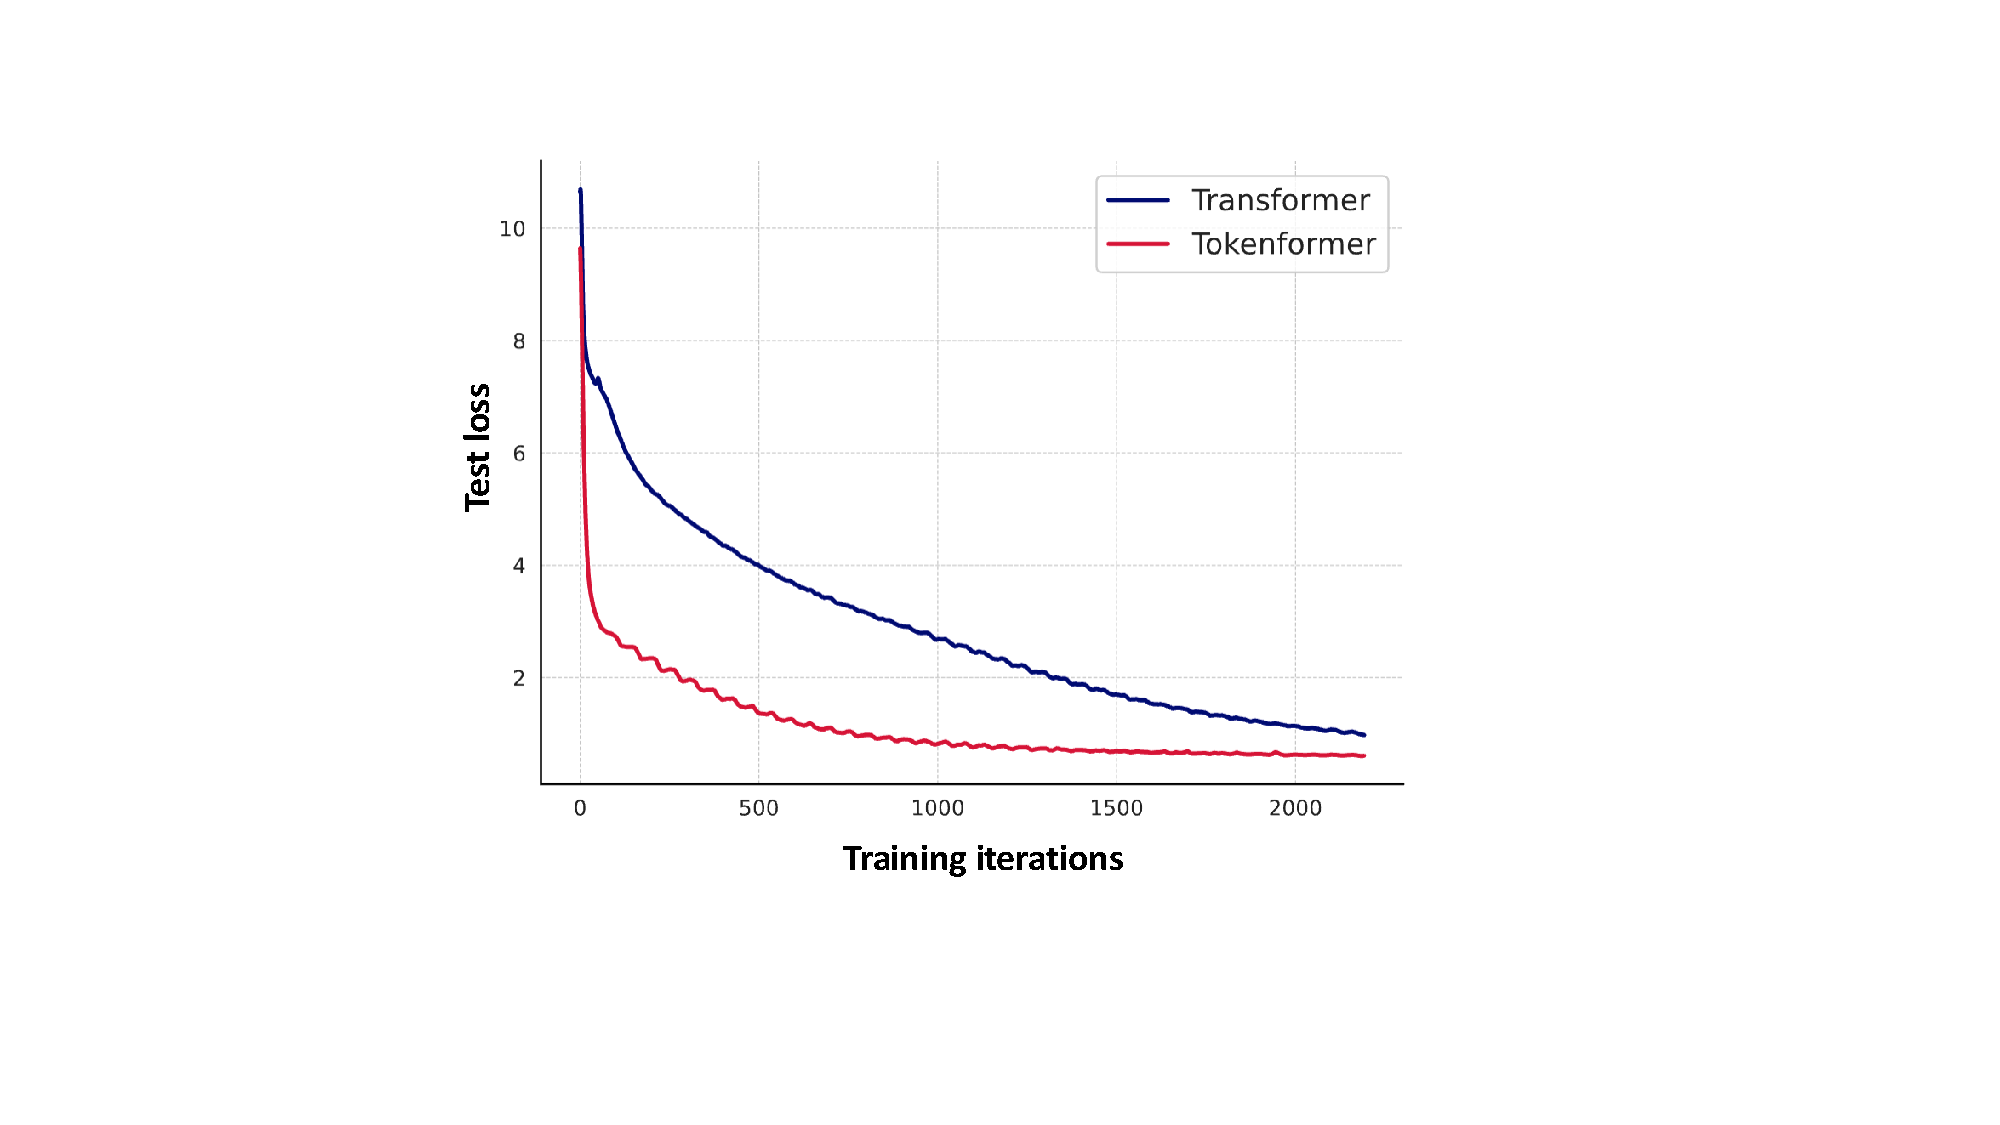
\includegraphics[width=\linewidth]{./transformer-paper/zero_init_v2.pdf}
      \caption{Loss curves comparing pre-trained Transformer and Tokenformer as their parameters are scaled during continued training on enwik8.}
      \label{fig:zero_init}
  \end{minipage}%
  \hfill
  \begin{minipage}{0.49\textwidth}
      \centering
      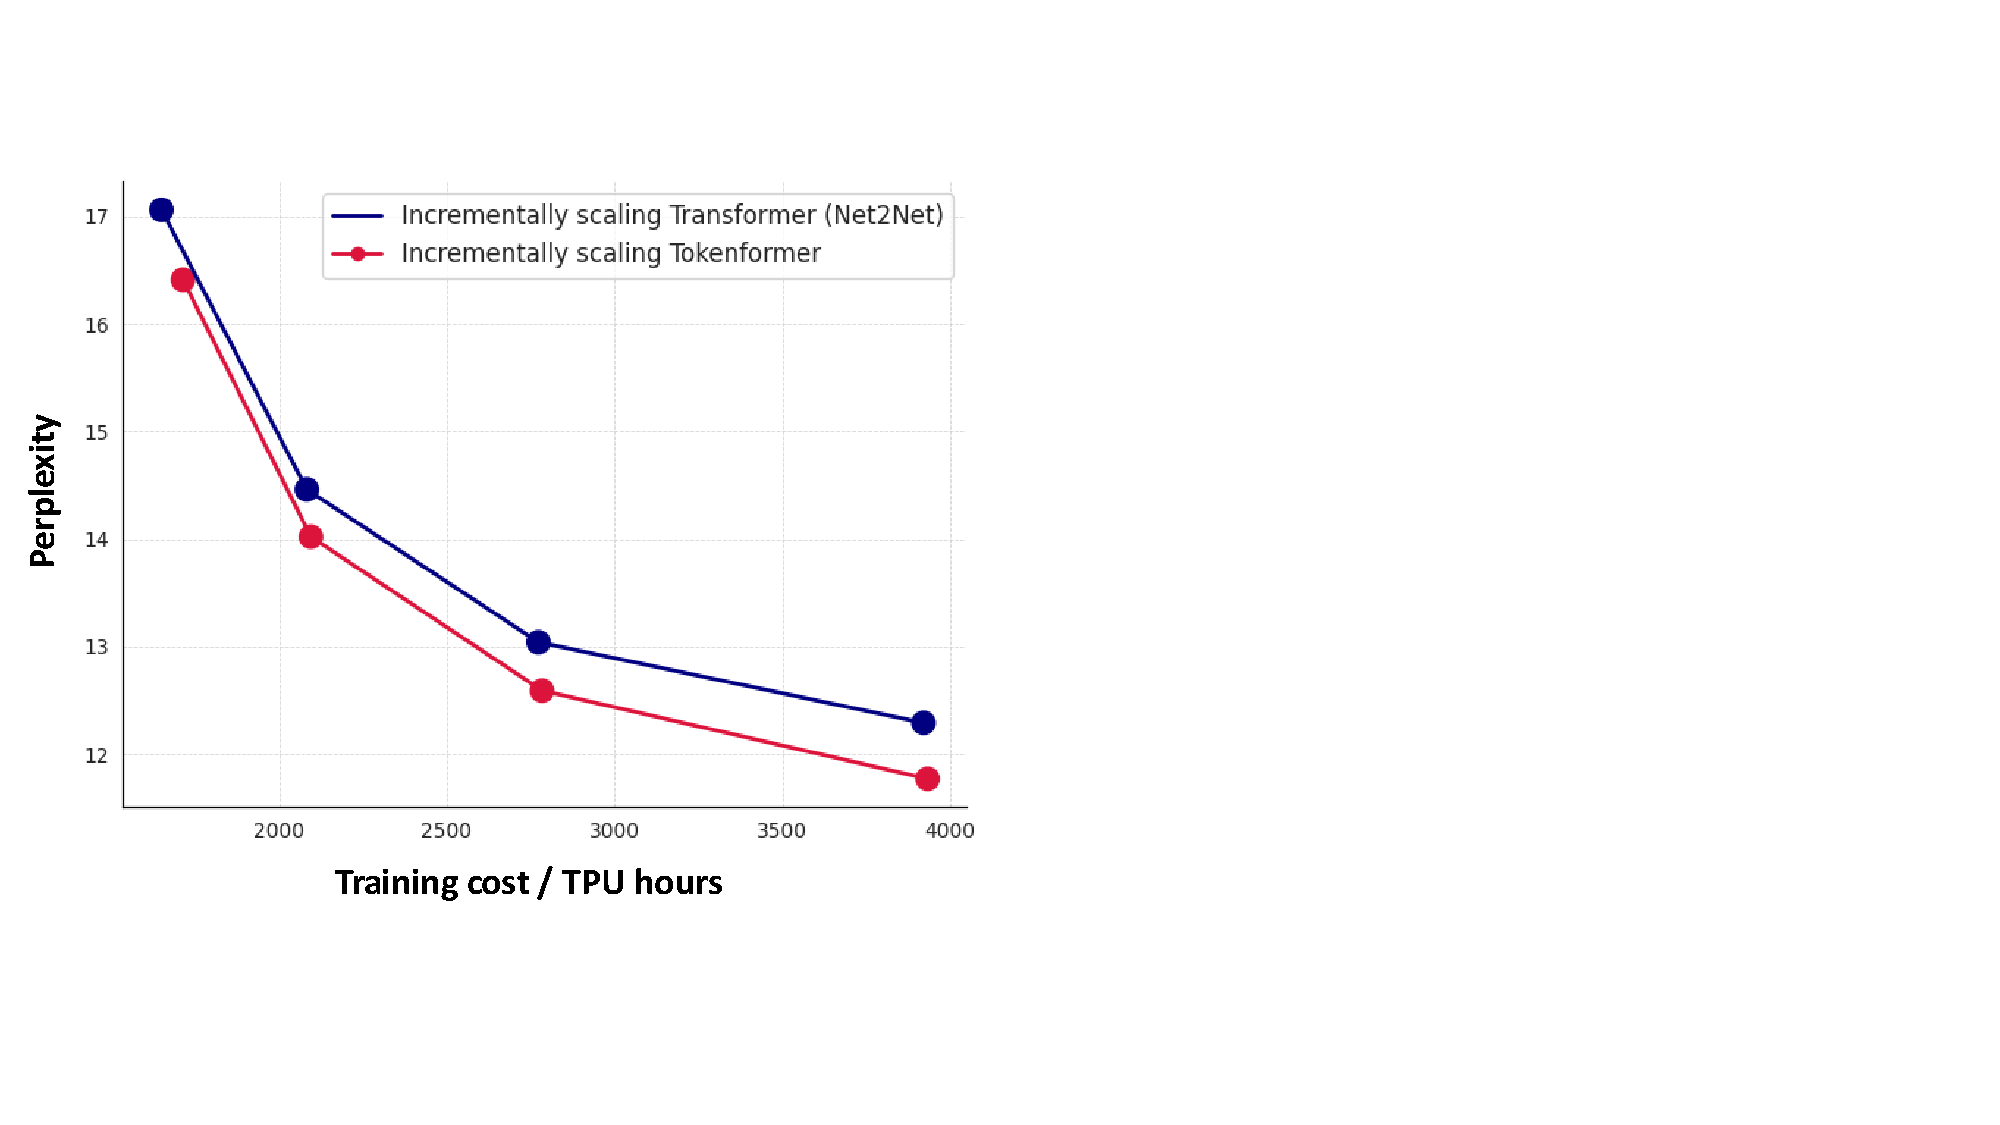
\includegraphics[width=\linewidth]{./transformer-paper/trans_vs_token.pdf}
      \caption{Performance benchmarking on incremental model scaling between Transformer with Net2Net scheme and Tokenformer.}
      \label{fig:comparision_tf_to}
  \end{minipage}
\end{figure}
\end{frame}


\section{Future Work}
\begin{frame}
\frametitle{Future Work}
\begin{itemize}
    \item \textbf{Advancing Parameter-Efficient Tuning.}
    When confronted with new tasks or datasets, the model can augment its pre-trained parameters
    by incorporating these new parameter tokens, thereby adapting to specific task requirements quickly.

    \item \textbf{Integrating Vision and Language Models.}
    Unify the key-value parameter tokens derived from pre-trained
    visual Tokeformer and language Tokenformer into a single parameter set.
    Then, introduce new learnable tokens to perform vision-language alignment
    and instruction tuning.
    
\end{itemize}
\end{frame}


% \section{介绍}
% \begin{frame}
% 	\frametitle{介绍}

% 	\begin{itemize}
% 		\item {编译方式}
% 		      \begin{itemize}
% 			      \item  推荐安装完整版的 TeXLive
% 			      \item 使用 \XeLaTeX 编译
% 		      \end{itemize}
% 		\item 请参考 \LaTeX 和 Beamer 用户文档

% 		\item 行内数学公式示例 $\sin^2 \theta + \cos^2 \theta = 1$
% 		\item {行间数学公式示例 \begin{equation}
% 			      y_{1}=\int \sin x\, {\rm d}x
% 		      \end{equation}	 }
% 		\item 基于“浙大蓝”颜色 \url{https://www.zju.edu.cn/}
% 	\end{itemize}
% \end{frame}

% \section{内置环境}
% \begin{frame}
% 	\frametitle{内置环境}
% 	\begin{block}{Slides with \LaTeX}
% 		Beamer offers a lot of functions to create nice slides using \LaTeX.
% 	\end{block}

% 	\begin{block}{The basis}
% 		内部使用以下主题
% 		\begin{itemize}
% 			\item split
% 			\item whale
% 			\item rounded
% 			\item orchid
% 		\end{itemize}
% 	\end{block}
% \end{frame}

% \begin{frame}
% 	\frametitle{带数字列表}
% 	\begin{enumerate}
% 		\item This just shows the effect of the style
% 		\item It is not a Beamer tutorial
% 		\item Read the Beamer manual for more help
% 		\item Contact me only concerning the style file
% 	\end{enumerate}
% \end{frame}

% \section{结论}
% \begin{frame}
% 	\frametitle{结论}

% 	\begin{itemize}
% 		\item Easy to use
% 		\item Good results
% 	\end{itemize}
% \end{frame}

% \section{参考文献}
% \begin{frame}{参考文献}
% 	\begin{thebibliography}{99}
% 		\bibitem{zhao1} Yi~Zhao, {\sl An introduction to X}, Sep.~15, 2015
% 		\bibitem{qian2} Er~Qian, San~Sun,
% 		Phys.\ Lett.\ A {\bf xx}, 2xx (20xx)
% 		\bibitem{li4} Si~Li, Phys.\ Rev.\ C {\bf xx}, 5xx (20xx)

% 	\end{thebibliography}
% \end{frame}

\end{document}